\documentclass{article}

% Language setting
% Replace `english' with e.g. `spanish' to change the document language
\usepackage[english]{babel}

% Set page size and margins
\usepackage[letterpaper,top=2cm,bottom=2cm,left=3cm,right=3cm,marginparwidth=1.75cm]{geometry}
% Useful packages
\usepackage{amsmath}
\usepackage{graphicx}
\usepackage{minted}
\usepackage[colorlinks=true, allcolors=blue]{hyperref}

\title{Homework 2 \\ Language Based Technology for Security} 
\author{Niccolo' Piazzesi \\ n.piazzesi@studenti.unipi.it}

\begin{document}
\maketitle

\section*{Introduction}
For this homework, i will present and discuss the paper "\textbf{MirChecker: Detecting Bugs in Rust Programs via Static Analysis}" by 
Zhuohua Li, Jincheng Wang, Mingshen Sun, and John C.S Lui \cite{li2021mirchecker}. This paper present a novel static analysis tool for the Rust programming language, 
focusing on detecting and preventing potential runtime crashes and memory safety bugs.
\section*{Paper Summary}
We can divide the paper in four parts: at the beginning, all the necessary background knowledge about static analysis and Rust 
is established, and the main motivations for the tool development are explained. Then, the high level design of the tool is presented, and the reasoning behind all the relevant choices is 
given. After that, the authors delve deeper in the actual implementation, showing the algorithm used and giving all the important technical details. The last part is about a series of benchmark used to 
test both the efficacy and speed of the developed tool on target examples. Finally, the authors discuss the achieved results, limitations, and the potential future directions of their work.
\subsection*{Background Knowledge and Motivations}
The paper begins by giving the basic knowledge needed to understand its results. The authors start by presenting all the necessary  theory and concepts of abstract interpretation. 
They recall the notions of \textbf{lattice} and \textbf{abstract transfer functions}, showing how they are  used to represent computations on abstract program states. 

In the next part, there is an introduction on the  main features of Rust, mainly about its 
powerful type and ownership system. It is mentioned how the restrictive rules for aliasing and mutability prevents many of the typical memory corruption problems. After, the main motivation for the work is presented: although 
Rust has very advanced tools for memory safety, their incomplete nature and the presence of the \mintinline{rust}{unsafe} keyword  can breach its safety promises, leading  to undetected bugs or worse, undefined behavior. The paper focus on two 
classes of issues affecting the language: \begin{itemize}
    \item \textbf{Runtime panics}.  Rust's type system cannot enforce all the security conditions statically. Some conditions such as array bounds checking or integer overflow detection are postponed until execution, with 
    the compiler automatically instrumenting assertions that, when violated, halt the program. Although this is still a safe way to handle these issues (no memory corruption is possible), an attacker could still exploit this 
    to cause denial of service.
    \item \textbf{Lifetime corruptions.} While  classical memory corruption bugs such as use-after-free or dangling pointers are well managed in Rust, using \mintinline{rust}{unsafe} and combining 
    it with the ownership system may lead to lifetime bugs where, first the unsafe code  causes invalid pointers or shared mutable memory, and then the ownership system automatically drops that memory, leading back to use after free bugs.
\end{itemize}
To prevent these issues, the authors decided to combine numerical static analysis to detect possible runtime panics generated by integer operations,
 and symbolic analysis to track heap memory ownership.
\subsection*{High level design}
MirChecker performs static analysis on top of Rust's Mid-level Intermediate Representation (MIR). MIR is produced as an intermediate step during normal compilation. 
It corresponds to a control flow graph (CFG) representation  and borrow checking is performed on it. Traditionally, Rust static analysis tools reason on LLVM IR or  a custom IR, but the authors decided to use MIR 
for two main reasons. First, while it reduces most of the complex syntax to a simpler core language, it preserves type information and debugging data, which is used to simplify the actual algorithm.
Second, LLVM API targets directly C/C++ and are then ported to Rust. Many compatibility issues may arise, differently from using 
a native representation. 


\paragraph*{Static analyzer}
\paragraph*{User interface} MirChecker is shipped as a cargo subcommand. 
Cargo is Rust's official package manager

\begin{minted}{bash}
    cargo mir-checker --\ 
    --entry <entry-function-name>\
    --domain <abstract-domain>\ 
    --widening_delay <N>\
    --narrowing_iteration <N>\ 
    --suppress_warnings <S>
\end{minted}
\begin{figure}[H]
    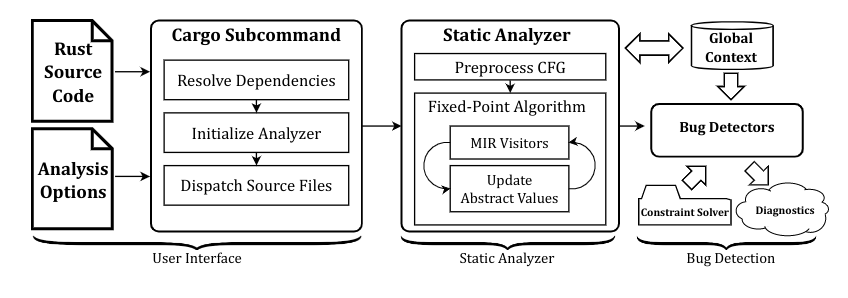
\includegraphics[scale=0.5]{hilev.png}
    \caption{High level view of Mir-Checker}
    \label{fig:hilev}
\end{figure}
\autoref{fig:hilev}
\subsection*{Implementation}
\subsection*{Benchmarks}

\section*{Advantages}

\section*{Disadvantages}

\section*{Possible Improvements}

\bibliographystyle{plain}
\bibliography{bib.bib}
\end{document}